\documentclass[12pt]{article}

\usepackage{graphicx}
\usepackage{geometry}
 \geometry{
 a4paper,
 total={170mm,257mm},
 left=20mm,
 top=20mm,
 }


\begin{document}


\title{MAKERERE UNIVERSITY\\ COLLEGE OF COMPUTING AND INFORMATION SCIENCES \\ A Report On  Makerere University Colleges}
\author{By Matovu Joseph | RegNo. 15/U/7462/PS | StudentNo.215011917} 
\maketitle


\begin{center}
EXECUTIVE SUMMARY\par
This Report is based on research about the colleges in makerere university. This involved collecting data about all colleges in makerere concerning location, schools in each college, name of the college and including site views of the colleges. The method used in this research was electronic data collection in which the ODK Build , ODK Collect  and ODK Aggregate Server tools were used in the gathering and organising of the data.  
\end{center}

\tableofcontents

\section{INTRODUCTION}
Makerere university has a number of colleges inwhich these colleges have branches called schools. These colleges and schools are located in various areas around makerere and in this case, many students and other people find difficulties locating and identifying them, and also differentiating the colleges from schools. This research aims at collecting information concerning all colleges in makerere university.

\section{BACKGROUND}
In the beginning, makerere university was composed of faculties which were not divided into other schools. But as courses increased to come up, the faculties became colleges and these colleges were divided into schools hence some were shifted to different locations around makerere. This brought in the problem of identifying colleges from schools and locating them. This research is aimed at solving this problem.

\section{AIM OF THE RESEARCH}
The main aim of this research is to come up with the neccessary information about all the colleges in makerere which is going to be needed during implentation of a system that will solve the problem of locating the different colleges and schools so as to provide quick knowledge to the students and other people in makerere.

\section{FINDINGS}
During the research, the following were the issues found out:-
\begin{itemize}
\item  	 Most students in makerere find difficulties locating some colleges and differentiating the colleges from schools.

\item	 Some Colleges and schools are very distant from each other and it take some long time to get to other colleges.

\item	 Some Junctions in makerere lack Posts to offer directions to those that may not be knowing some directions to other colleges.


\end{itemize}

\section{METHODOLOGY}
The research was done using electronic methods. This involved using the OpenData Kit Build (ODK Build) to build the form that looks like a questionnier depending on the data need in the research. This ODK Build provides an Extensible Mark-up Language (xml) form format which is uploaded to the Aggregate Server that receives the research data sent using the ODK Collect application on the mobile device. The ODK Collect Application is able to do this through uploading the created xml form into it and connecting the ODK Aggregate Server to the ODK Collect using the Aggregate server url. The Aggregate server store all the informing being collected and sent to it.

\subsection{ODK COLLECT APPLICATION DATA VIEW}

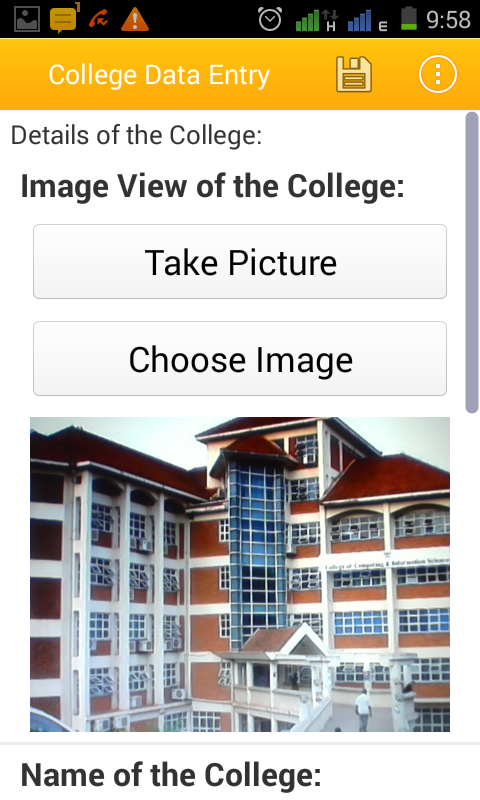
\includegraphics[width=0.3\linewidth, height=6cm]{datacollect}\\

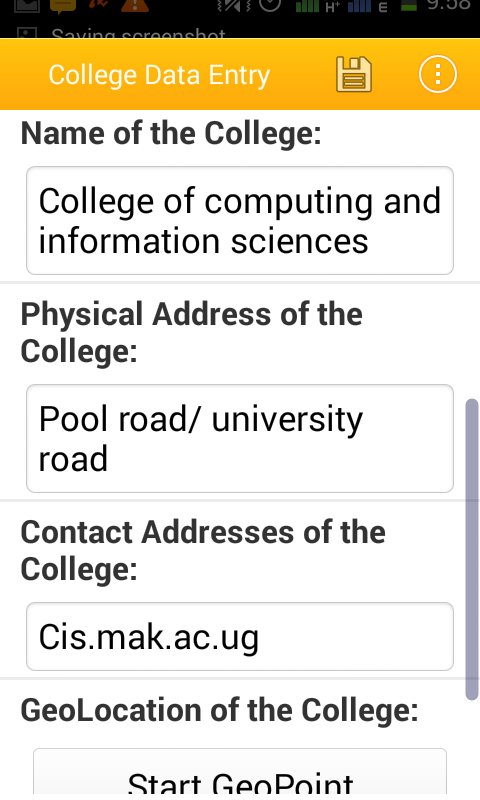
\includegraphics[width=0.3\linewidth, height=6cm]{datacollect1}



\subsection{ODK AGGREGATE SERVER VIEW }

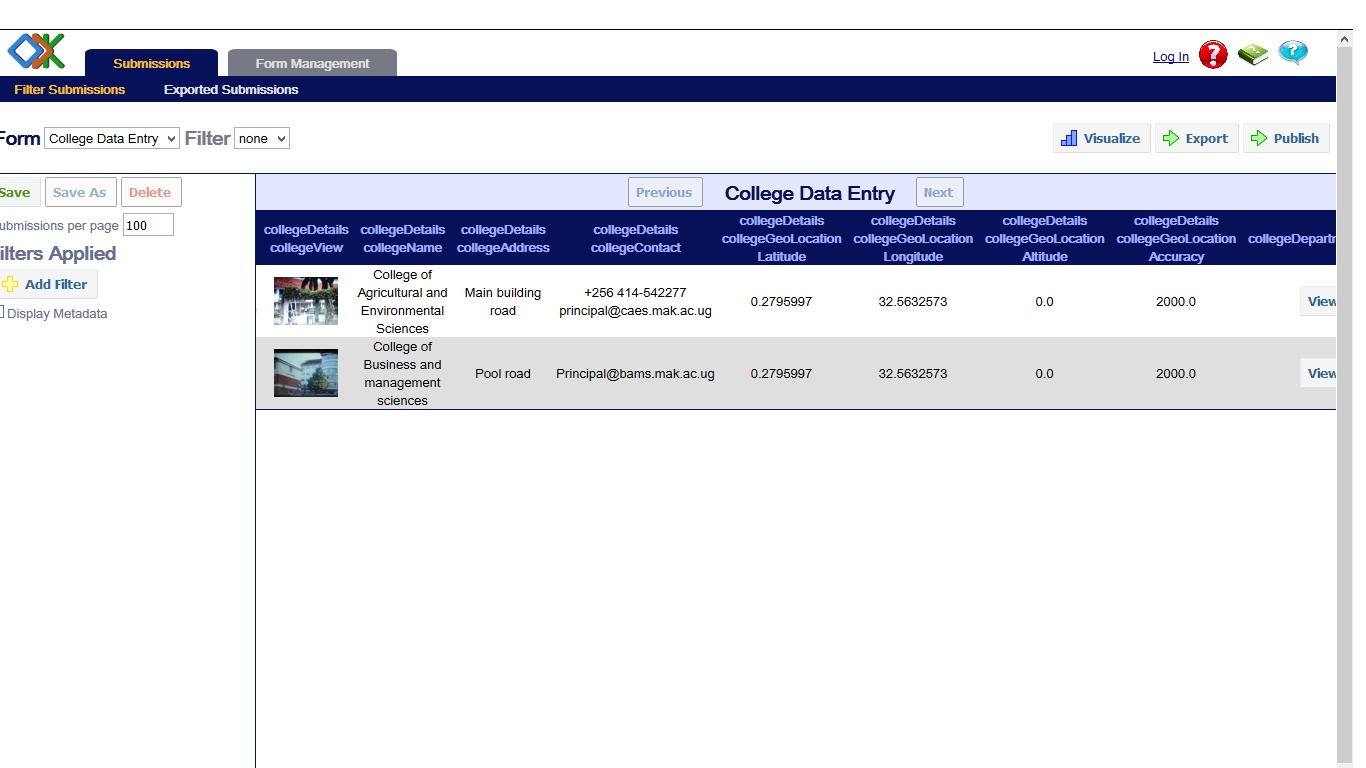
\includegraphics[width=0.9\linewidth, height=5cm]{serverView}

\section{CONCLUSION}
During this research about the  colleges in makerere, i realized that many students don't know where some colleges are located , and have never seen them apart from just hearing them. With the data collected through this research, every student and persons within makerere will be able to locate and know about every college in makerere.

\section{REFERENCES}

[1] Aggregate server base, url:datacollection-168008.appspot.com ; Data collected about the makerere university colleges

[2] Mak thru; An application on google play. 


\end{document}